\documentclass[]{article}

% Imported Packages
%------------------------------------------------------------------------------
\usepackage{amssymb}
\usepackage{amstext}
\usepackage{amsthm}
\usepackage{amsmath}
\usepackage{enumerate}
\usepackage{fancyhdr}
\usepackage[margin=1in]{geometry}
\usepackage{graphicx}
\usepackage{float}
%\usepackage{extarrows}
%\usepackage{setspace}
%------------------------------------------------------------------------------

% Header and Footer
%------------------------------------------------------------------------------
\pagestyle{plain}  
\renewcommand\headrulewidth{0.4pt}                                      
\renewcommand\footrulewidth{0.4pt}                                    
%------------------------------------------------------------------------------

% Title Details
%------------------------------------------------------------------------------
\title{Deliverable \#2 Template}
\author{SE 3A04: Software Design II -- Large System Design}
\date{}                               
%------------------------------------------------------------------------------

% Document
%------------------------------------------------------------------------------
\begin{document}

\newcommand{\introduction}{
\newpage
\section{Introduction}
\label{sec:introduction}
% Begin Section

\subsection{Purpose}
\label{sub:purpose}
% Begin SubSection
The purpose of this document is to describe the high-level architecture of \textbf{SCEMAS} and explain how the system will be organized into subsystems with clear responsibilities and interactions. \\
\\
This document is intended for developers, system architects, project stakeholders, and instructors involved in the design and implementation of \textbf{SCEMAS}. It provides an overview of the architectural approach used in the system and serves as a reference for future development activities.
The document builds upon the requirements defined in the Software Requirements Specification (Deliverable 1) and translates those requirements into a structured architectural design.% End SubSection

\subsection{System Description}
\label{sub:system_description}
% Begin SubSection
The system uses a \textbf{Presentation–Abstraction–Control (PAC)} architectural style. 
This consists of presentation, control and abstraction components. Presentation handles user interfaces and interaction, abstraction has the control and data management, and control coordinates between the other two layers and other agents.\\ \\
The various subsystems use the following architectural styles: repository, pipe-and-filter, and blackboard. 
Repository allows the subsystem to manage account information and \textbf{RBAC}. 
Pipe-and-filter allows the subsystem to process sensor data through various stages.
Blackboard allows incoming telemetry to be compared against set values to create alerts.
These architectural styles were chosen to promote modularity and maintainability, allowing the system to be organized into cohesive subsystems.

% End SubSection

\subsection{Overview}
\label{sub:overview}
% Begin SubSection
The rest of the document describes the architectural design of \textbf{\textbf{SCEMAS}}, including the high-level structure of the system, the main components and their interactions, and the rationale behind the architectural decisions. The document is organized as follows:
Section 2 is the Analysis Class Diagram, which identifies important classes and their relationships.
Section 3 is Architectural Design, which identifies the system architecture, subsystems, and provides justification for design choices.
Section 4 contains the Class Responsibility Collaborator (CRC) cards, which provide detailed information about the responsibilities and interactions of the main classes in the system.
% End SubSection

}
\newcommand{\analysis}{
\section{Analysis Class Diagram}
\label{sec:analysis_class_diagram}
% Begin Section
    \begin{figure}[h!]
        \centering
        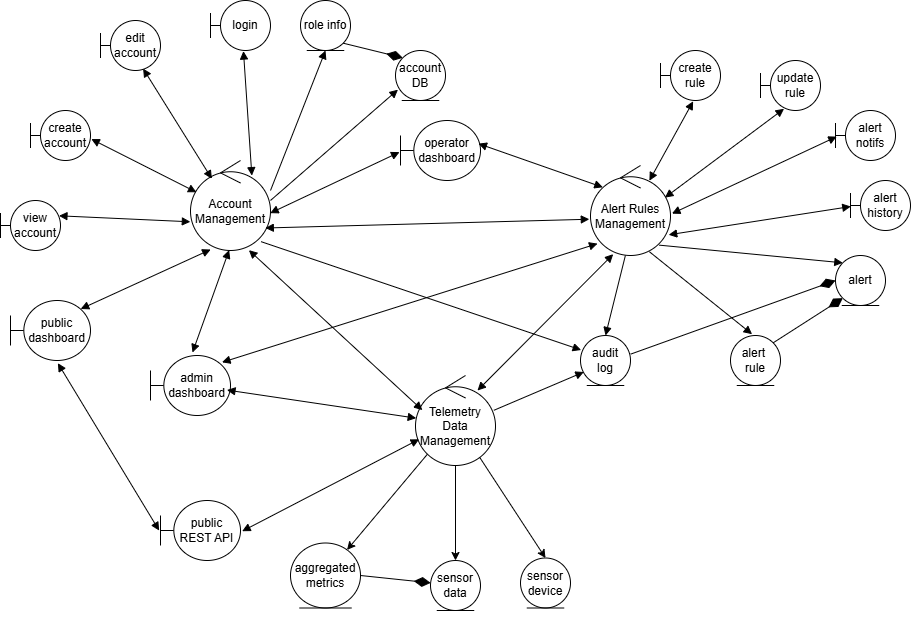
\includegraphics[width=1.1\linewidth]{AnalysisClassDiagram.png}
        \caption{Analysis Class Diagram}
    \end{figure}

}
\newcommand{\architectural}{

\section{Architectural Design}
\label{sec:architectural_design}
% Begin Section
This section should provide an overview of the overall architectural design of your application. Your overall architecture should show the division of the system into subsystems with high cohesion and low coupling.

\subsection{System Architecture}
\label{sub:system_architecture}
% Begin SubSection
% \begin{itemize}
% 	\item Identify and explain the overall architecture of your system
% 	\item Be sure to clearly state the name of the architecture you used (this is the name of the architectural pattern, not the name of your system)
% 	\item Provide the reasoning and justification of the choice of architecture
% 	\item Provide a structural architecture diagram showing the relationship among the subsystems (if appropriate)
% 	\item List any design alternatives you considered, but eliminated (and explain why you eliminated them)
% \end{itemize} \\

\noindent SCEMAS utilizes the \textbf{Presentation–Abstraction–Control (PAC)} architectural style. In PAC, the system is divided into a set of cooperating agents. Each agent contains three components: presentation, control, and abstraction. The presentation component handles user interaction and external interfaces, the abstraction component contains the system’s data and core logic, and the control component manages communication between presentation and abstraction while coordinating interactions between agents. \\

\noindent The top-level PAC agent represents the overall system and coordinates interactions between the system interfaces and internal subsystems. The presentation component provides entry points for the operator dashboard, administrative tools, and the public REST API. The control component routes requests to the appropriate subsystem agents and manages system-wide coordination. The abstraction component represents the overall system functionality and provides access to the core services of the system. \\

\noindent Within this architecture, several subsystem agents are defined. Each subsystem agent encapsulates its own presentation, control, and abstraction components while performing a specific system responsibility. 

\begin{itemize}

    \item The \textbf{Account Management} subsystem follows a \textbf{Repository} architectural style. This subsystem handles user accounts, authentication, and role-based access control. Account data is stored in a centralized repository so that different parts of the system can access and update user information consistently. 

    \item The \textbf{Telemetry Data Management} subsystem follows a \textbf{Pipe-and-Filter} architectural style. Telemetry data from IoT sensors is processed through a sequence of stages such as ingestion, validation, aggregation, and storage. Each stage acts as a filter that transforms the incoming data before passing it to the next stage through a pipe. This approach works well for telemetry data because it allows continuous data streams to be processed efficiently. 

    \item The \textbf{Alert Rules Management} subsystem follows a \textbf{Blackboard} architectural style. In this subsystem, incoming telemetry data is evaluated against administrator-defined alert rules. The blackboard serves as a shared knowledge base containing telemetry values and alert rules. Multiple components can operate on this shared data to determine whether environmental thresholds have been exceeded and to generate alerts. 

\end{itemize}

\noindent Alternative architectures were considered but ultimately eliminated. The Model–View–Controller (MVC) architecture was considered because it separates the user interface from the application logic. However, MVC is typically suited for systems centered around a single interface and shared data model. Since SCEMAS contains independent processing subsystems, PAC provides a clearer way to coordinate these components. The Batch Sequential architecture was not suitable because SCEMAS requires continuous real-time processing of telemetry data rather than batch processing. The Process-Control architecture is primarily used in embedded systems that directly control hardware processes, which is not the main purpose of SCEMAS. \\

% End SubSection

\subsection{Subsystems}
\label{sub:subsystems}
% Begin SubSection
\noindent Provide a list of your subsystems, with a brief description of each. Be sure to document its purpose and relationship to other subsystems. \\

\noindent Our main system has been subdivided into three distinct subsystems: Telemetry Data Management, Account Management, and Alert Rules Management. Each subsystem is designed to handle specific responsibilities while maintaining clear interfaces for communication with other subsystems. \\

\noindent The Telemetry Data Management subsystem is responsible for handling the ingestion, processing, and storage of telemetry data from IoT sensors. It ensures that incoming data is validated, aggregated, and stored efficiently for later retrieval and analysis. This subsystem adheres to a pipe-and-filter architectural style and interacts with the Alert Rules Management subsystem to evaluate telemetry data against defined alert rules. \\

\noindent The Account Management subsystem manages user accounts, authentication, and role-based access control. It provides a centralized repository for user information and ensures that only authorized users can access specific system functionalities. This subsystem interacts with both the Telemetry Data Management and Alert Rules Management subsystems to enforce access control policies. The Account Management System is built on the repository architectural style, allowing for consistent data access and updates across the system. \\

\noindent The Alert Rules Management subsystem allows administrators to define and manage alert rules based on telemetry data. It evaluates telemetry data from the Telemetry Data Management subsystem against these rules and generates alerts when certain conditions are met. This subsystem uses a blackboard architectural style to allow administrators to share alert conditions across the system. \\
% End SubSection
}
\newcommand{\crc}{
\section{Class Responsibility Collaboration (CRC) Cards}
\label{sec:class_responsibility_collaboration_crc_cards}
% Begin Section
This section should contain all of your CRC cards.

\begin{itemize}
	\item Provide a CRC Card for each identified class
	\item Please use the format outlined in tutorial, i.e., 
	\begin{table}[ht]
		\centering
		\begin{tabular}{|p{8cm}|p{8cm}|}
		\hline 
		 \multicolumn{2}{|l|}{\textbf{Class Name:} Account Management (Controller)} \\
		\hline 
		\textbf{Responsibility:} & \textbf{Collaborators:} \\
		\hline
		 - Knows Create Account & - Create Account \\
		 - Knows Edit Account & - Edit Account \\
		 - Knows Login & - Login \\
		 - Knows Role Info & - Role Info \\
		 - Knows Account DB & - Account DB \\
		 - Knows Operator Dashboard & - Operator Dashboard \\
		 - Knows Alert Rules Management & - Alert Rules Management \\
		 - Knows Audit Log & - Audit Log \\
		 - Knows Telemetry Data Management & - Telemetry Data Management \\
		 - Knows Admin Dashboard & - Admin Dashboard \\
		 - Knows Public Dashboard & - Public Dashboard \\
		 - Knows View Account & - View Account \\
		\hline
		\end{tabular}
	\end{table}


	\begin{table}[ht]
		\centering
		\begin{tabular}{|p{8cm}|p{8cm}|}
		\hline 
		 \multicolumn{2}{|l|}{\textbf{Class Name:} Alert Rules Management (Controller)} \\
		\hline
		\textbf{Responsibility:} & \textbf{Collaborators:} \\
		\hline
		 - Knows Create Rule & - Create Rule \\
		 - Knows Update Rule & - Update Rule \\
		 - Knows Alert Notifs & - Alert Notifs \\
		 - Knows Alert History & - Alert History \\
		 - Knows Alert & - Alert \\
		 - Knows Alert Rule & - Alert Rule \\
		 - Knows Audit Log & - Audit Log \\
		 - Knows Telemetry Data Management & - Telemetry Data Management \\
		 - Knows Admin Dashboard & - Admin Dashboard \\
		 - Knows Account Management & - Account Management \\
		 - Knows Operator Dashboard & - Operator Dashboard \\
		\vspace{1in} & \\
		\hline
		\end{tabular}
	\end{table}

	\begin{table}[ht]
		\centering
		\begin{tabular}{|p{8cm}|p{8cm}|}
		\hline 
		 \multicolumn{2}{|l|}{\textbf{Class Name:} Telemetry Data Management (Controller)} \\
		\hline
		\textbf{Responsibility:} & \textbf{Collaborators:} \\
		\hline
		 - Knows Alert Rules Management & - Alert Rules Management \\
		 - Knows Audit Log & - Audit Log \\
		 - Knows Sensor Device & - Sensor Device \\
		 - Knows Sensor Data & - Sensor Data \\
		 - Knows Aggregated Metrics & - Aggregated Metrics \\
		 - Knows Public REST API & - Public REST API \\
		 - Knows Admin Dashboard & - Admin Dashboard \\
		 - Knows Account Management & - Account Management \\
		\vspace{1in} & \\
		\hline
		\end{tabular}
	\end{table}

	\begin{table}[ht]
		\centering
		\begin{tabular}{|p{8cm}|p{8cm}|}
		\hline 
		 \multicolumn{2}{|l|}{\textbf{Class Name:} Create Account (Boundary)} \\
		\hline
		\textbf{Responsibility:} & \textbf{Collaborators:} \\
		\hline
		 - Knows Account Management & - Account Management \\
		 - Handles click-event of "Create" button \\
		\vspace{1in} & \\
		\hline
		\end{tabular}
	\end{table}

	\begin{table}[ht]
		\centering
		\begin{tabular}{|p{8cm}|p{8cm}|}
		\hline 
		 \multicolumn{2}{|l|}{\textbf{Class Name:} Edit Account (Boundary)} \\
		\hline
		\textbf{Responsibility:} & \textbf{Collaborators:} \\
		\hline
		 - Knows Account Management & - Account Management \\
		 - Handles click-event of "Edit" button \\
		\vspace{1in} & \\
		\hline
		\end{tabular}
	\end{table}

	\begin{table}[ht]
		\centering
		\begin{tabular}{|p{8cm}|p{8cm}|}
		\hline 
		 \multicolumn{2}{|l|}{\textbf{Class Name:} Login (Boundary)} \\
		\hline
		\textbf{Responsibility:} & \textbf{Collaborators:} \\
		\hline
		 - Knows Account Management & - Account Management \\
		 - Handles click-event of "Login" button \\
		\vspace{1in} & \\
		\hline
		\end{tabular}
	\end{table}

	\begin{table}[ht]
		\centering
		\begin{tabular}{|p{8cm}|p{8cm}|}
		\hline 
		 \multicolumn{2}{|l|}{\textbf{Class Name:} View Account (Boundary)} \\
		\hline
		\textbf{Responsibility:} & \textbf{Collaborators:} \\
		\hline
		 - Knows Account Management & - Account Management \\
		 - Handles click-event of "View Account" button \\
		\vspace{1in} & \\
		\hline
		\end{tabular}
	\end{table}

	\begin{table}[ht]
		\centering
		\begin{tabular}{|p{8cm}|p{8cm}|}
		\hline 
		 \multicolumn{2}{|l|}{\textbf{Class Name:} Public Dashboard (Boundary)} \\
		\hline
		\textbf{Responsibility:} & \textbf{Collaborators:} \\
		\hline
		 - Knows Account Management & - Account Management \\
		 - Handles click-event of "View Public Dashboard" button \\
		\vspace{1in} & \\
		\hline
		\end{tabular}
	\end{table}

	\begin{table}[ht]
		\centering
		\begin{tabular}{|p{8cm}|p{8cm}|}
		\hline 
		 \multicolumn{2}{|l|}{\textbf{Class Name:} Admin Dashboard (Boundary)} \\
		\hline
		\textbf{Responsibility:} & \textbf{Collaborators:} \\
		\hline
		 - Knows Account Management & - Account Management \\
		 - Handles click-event of "View Admin Dashboard" button \\
		\vspace{1in} & \\
		\hline
		\end{tabular}
	\end{table}

	\begin{table}[ht]
		\centering
		\begin{tabular}{|p{8cm}|p{8cm}|}
		\hline 
		 \multicolumn{2}{|l|}{\textbf{Class Name:} Operator Dashboard (Boundary)} \\
		\hline
		\textbf{Responsibility:} & \textbf{Collaborators:} \\
		\hline
		 - Knows Account Management & - Account Management \\
		 - Handles click-event of "View Operator Dashboard" button \\
		\vspace{1in} & \\
		\hline
		\end{tabular}
	\end{table}

	\begin{table}[ht]
		\centering
		\begin{tabular}{|p{8cm}|p{8cm}|}
		\hline 
		 \multicolumn{2}{|l|}{\textbf{Class Name:} Public REST API (Boundary)} \\
		\hline
		\textbf{Responsibility:} & \textbf{Collaborators:} \\
		\hline
		 - Knows Telemetry Data Management & - Telemetry Data Management \\
		 - Handles API calls for telemetry data \\ 
		\vspace{1in} & \\
		\hline
		\end{tabular}
	\end{table}


	\begin{table}[ht]
		\centering
		\begin{tabular}{|p{8cm}|p{8cm}|}
		\hline 
		 \multicolumn{2}{|l|}{\textbf{Class Name:} Alert History (Boundary)} \\
		\hline
		\textbf{Responsibility:} & \textbf{Collaborators:} \\
		\hline
		 - Knows Telemetry Data Management & - Telemetry Data Management \\
		 - Handles click-event of "View Alert History" button\\ 
		\vspace{1in} & \\
		\hline
		\end{tabular}
	\end{table}

	\begin{table}[ht]
		\centering
		\begin{tabular}{|p{8cm}|p{8cm}|}
		\hline 
		 \multicolumn{2}{|l|}{\textbf{Class Name:} Alert Notifs (Boundary)} \\
		\hline
		\textbf{Responsibility:} & \textbf{Collaborators:} \\
		\hline
		 - Knows Telemetry Data Management & - Telemetry Data Management \\
		 - Handles click-event of "View Alert Notifs" button\\ 
		\vspace{1in} & \\
		\hline
		\end{tabular}
	\end{table}

	\begin{table}[ht]
		\centering
		\begin{tabular}{|p{8cm}|p{8cm}|}
		\hline 
		 \multicolumn{2}{|l|}{\textbf{Class Name:} Update Rule (Boundary)} \\
		\hline
		\textbf{Responsibility:} & \textbf{Collaborators:} \\
		\hline
		 - Knows Telemetry Data Management & - Telemetry Data Management \\
		 - Handles click-event of "Update Rule" button\\ 
		\vspace{1in} & \\
		\hline
		\end{tabular}
	\end{table}

	\begin{table}[ht]
		\centering
		\begin{tabular}{|p{8cm}|p{8cm}|}
		\hline 
		 \multicolumn{2}{|l|}{\textbf{Class Name:} Create Rule (Boundary)} \\
		\hline
		\textbf{Responsibility:} & \textbf{Collaborators:} \\
		\hline
		 - Knows Telemetry Data Management & - Telemetry Data Management \\
		 - Handles click-event of "Create Rule" button\\ 
		\vspace{1in} & \\
		\hline
		\end{tabular}
	\end{table}

	\begin{table}[ht]
		\centering
		\begin{tabular}{|p{8cm}|p{8cm}|}
		\hline 
		 \multicolumn{2}{|l|}{\textbf{Class Name:} Role Info (Entity)} \\
		\hline
		\textbf{Responsibility:} & \textbf{Collaborators:} \\
		\hline
		 - Knows Account  Management & - Account Management \\
		\vspace{1in} & \\
		\hline
		\end{tabular}
	\end{table}

	\begin{table}[ht]
		\centering
		\begin{tabular}{|p{8cm}|p{8cm}|}
		\hline 
		 \multicolumn{2}{|l|}{\textbf{Class Name:} Account DB (Entity)} \\
		\hline
		\textbf{Responsibility:} & \textbf{Collaborators:} \\
		\hline
		 - Knows Account  Management & - Account Management \\
		 - Knows Role Info & - Role Info \\
		\vspace{1in} & \\
		\hline
		\end{tabular}
	\end{table}

	\begin{table}[ht]
		\centering
		\begin{tabular}{|p{8cm}|p{8cm}|}
		\hline 
		 \multicolumn{2}{|l|}{\textbf{Class Name:} Aggregated Metrics (Entity)} \\
		\hline
		\textbf{Responsibility:} & \textbf{Collaborators:} \\
		\hline
		 - Knows Telemetry Data Management & - Telemetry Data Management \\
		\vspace{1in} & \\
		\hline
		\end{tabular}
	\end{table}

	\begin{table}[ht]
		\centering
		\begin{tabular}{|p{8cm}|p{8cm}|}
		\hline 
		 \multicolumn{2}{|l|}{\textbf{Class Name:} Sensor Data (Entity)} \\
		\hline
		\textbf{Responsibility:} & \textbf{Collaborators:} \\
		\hline
		 - Knows Telemetry Data Management & - Telemetry Data Management \\
		 - Knows Aggregated Metrics & - Aggregated Metrics \\
		\vspace{1in} & \\
		\hline
		\end{tabular}
	\end{table}

	\begin{table}[ht]
		\centering
		\begin{tabular}{|p{8cm}|p{8cm}|}
		\hline 
		 \multicolumn{2}{|l|}{\textbf{Class Name:} Sensor Device (Entity)} \\
		\hline
		\textbf{Responsibility:} & \textbf{Collaborators:} \\
		\hline
		 - Knows Telemetry Data Management & - Telemetry Data Management \\
		\vspace{1in} & \\
		\hline
		\end{tabular}
	\end{table}

	\begin{table}[ht]
		\centering
		\begin{tabular}{|p{8cm}|p{8cm}|}
		\hline 
		 \multicolumn{2}{|l|}{\textbf{Class Name:} Audit Log (Entity)} \\
		\hline
		\textbf{Responsibility:} & \textbf{Collaborators:} \\
		\hline
		 - Knows Alert Rules Management & - Alert Rules Management \\
		 - Knows Account Management & - Account Management \\
		 - Knows Telemetry Data Management & - Telemetry Data Management \\
		\vspace{1in} & \\
		\hline
		\end{tabular}
	\end{table}

	\begin{table}[ht]
		\centering
		\begin{tabular}{|p{8cm}|p{8cm}|}
		\hline 
		 \multicolumn{2}{|l|}{\textbf{Class Name:} Alert Rule (Entity)} \\
		\hline
		\textbf{Responsibility:} & \textbf{Collaborators:} \\
		\hline
		 - Knows Alert Rules Management & - Alert Rules Management \\
		\vspace{1in} & \\
		\hline
		\end{tabular}
	\end{table}

	\begin{table}[ht]
		\centering
		\begin{tabular}{|p{8cm}|p{8cm}|}
		\hline 
		 \multicolumn{2}{|l|}{\textbf{Class Name:} Alert (Entity)} \\
		\hline
		\textbf{Responsibility:} & \textbf{Collaborators:} \\
		\hline
		 - Knows Alert Rules Management & - Alert Rules Management \\
		 - Knows Audit Log & - Audit Log \\
		 - Knows Alert Rule & - Alert Rule \\
		\vspace{1in} & \\
		\hline
		\end{tabular}
	\end{table}


\end{itemize}
}

\maketitle	
\noindent{\bf Tutorial Number:} T02\\
{\bf Group Number:} G3 \\
{\bf Group Members:} Resham Vani, Sama Al-Oda, Ranvir Jhajj, Patrick Molka, Atharva Kulkarni

\section*{IMPORTANT NOTES}
\begin{itemize}
	%	\item You do \underline{NOT} need to provide a text explanation of each diagram; the diagram should speak for itself
	\item Please document any non-standard notations that you may have used
	\begin{itemize}
		\item \emph{Rule of Thumb}: if you feel there is any doubt surrounding the meaning of your notations, document them
	\end{itemize}
	\item Some diagrams may be difficult to fit into one page
	\begin{itemize}
		\item Ensure that the text is readable when printed, or when viewed at 100\% on a regular laptop-sized screen.
		\item If you need to break a diagram onto multiple pages, please adopt a system of doing so and thoroughly explain how it can be reconnected from one page to the next; if you are unsure about this, please ask about it
	\end{itemize}
	\item Please submit the latest version of Deliverable 1 with Deliverable 2
	\begin{itemize}
		\item Indicate any changes you made.
	\end{itemize}
	\item If you do \underline{NOT} have a Division of Labour sheet, your deliverable will \underline{NOT} be marked
\end{itemize}

\introduction

% End Section

\analysis

% End Section

\architectural

% End Section

\crc

% End Section

\appendix
\section{Division of Labour}
\label{sec:division_of_labour}
% Begin Section

{\bf Resham Vani}
\begin{itemize}
	\item 2
\end{itemize}

\begin{figure}[H]
    
\includegraphics[width=0.2\linewidth]{../deliverable 1/Resham_Signature.png}
\end{figure}

{\bf Sama Al-Oda}
\begin{itemize}
	\item 4
\end{itemize}

\begin{figure}[H]
    
\includegraphics[width=0.2\linewidth]{../deliverable 1/Sama_Signature.png}
\end{figure}

{\bf Patrick Molka}
\begin{itemize}
	\item 3.2
\end{itemize}

\begin{figure}[H]
    
\includegraphics[width=0.2\linewidth]{../deliverable 1/Patrick_Signature.png}
\end{figure}

{\bf Atharva Kulkarni}
\begin{itemize}
	\item 3.1
\end{itemize}

\begin{figure}[H]
    
\includegraphics[width=0.2\linewidth]{../deliverable 1/Atharva_Signature.png}
\end{figure}

{\bf Ranvir Jhajj}
\begin{itemize}
	\item 1
\end{itemize}

\begin{figure}[h!]
    
\includegraphics[width=0.3\linewidth]{../deliverable 1/Ranvir_Signature.png}
\end{figure}

% End Section


\end{document}
%------------------------------------------------------------------------------